\pagestyle{fancy}
\chapter{\heiti 软件安装}
\setmainfont{Times New Roman}

我司会为用户提供“ASG\_install”文件夹,里面包含安装仪器控制软件所需的所有文件。

\section{Python\heiti 解释器安装}
用户可到Python官网(http://www.python.org/)下载Python 2.7版本的解释器(推荐下载32位),也可直接双击运行我司提供的“ASG\_install”文件夹下“Python-2.7.11.msi”安装程序,在选择安装组件的一步时,务必勾选所有组件,然后点击“Next”即可完成安装,计算机默认会将Python解释器安装到C:\textbackslash Python27 目录下。安装完成后,打开命令提示符窗口,输入“Python” 后,如果出现如图3.1所示情况,则代表Python解释器安装成功。若得到“Python不是内部或外部命令,也不是可运行的程序或批处理文件”,请右键“计算机” → “属性” →“ 系统高级设置” →“ 高级” → “环境变量”,然后在系统变量中找到Path,编辑此变量在后面追加“;C:\textbackslash python(python安装位置)”。如果仍未安装成功,建议把Python安装程序重新运行一遍,记得勾选Add python.exe to Path。
%\begin{figure}[ht]
%\centering
%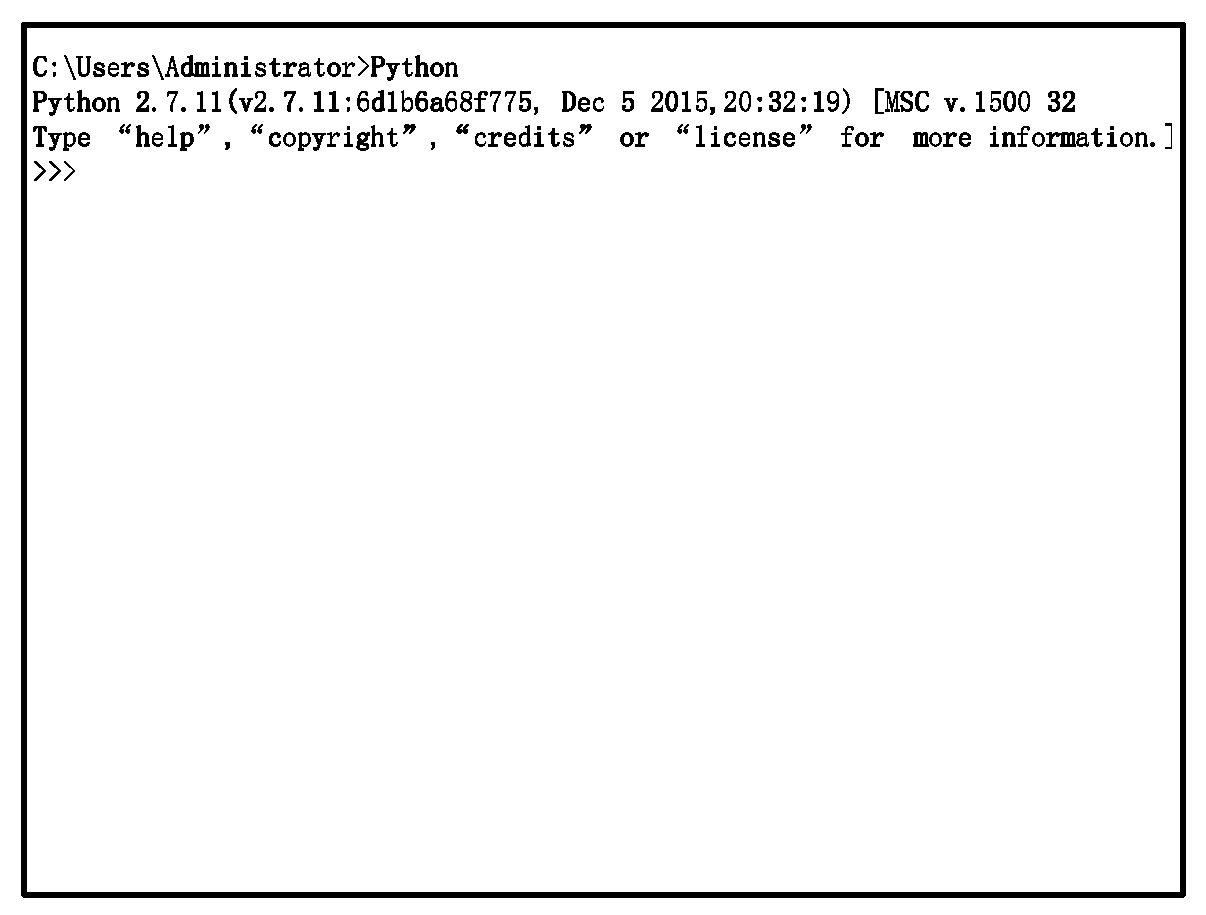
\includegraphics[width=10cm]{fig3_1}
%\caption{Python 安装勾选组件}
%\end{figure}
\begin{figure}[ht]
\centering
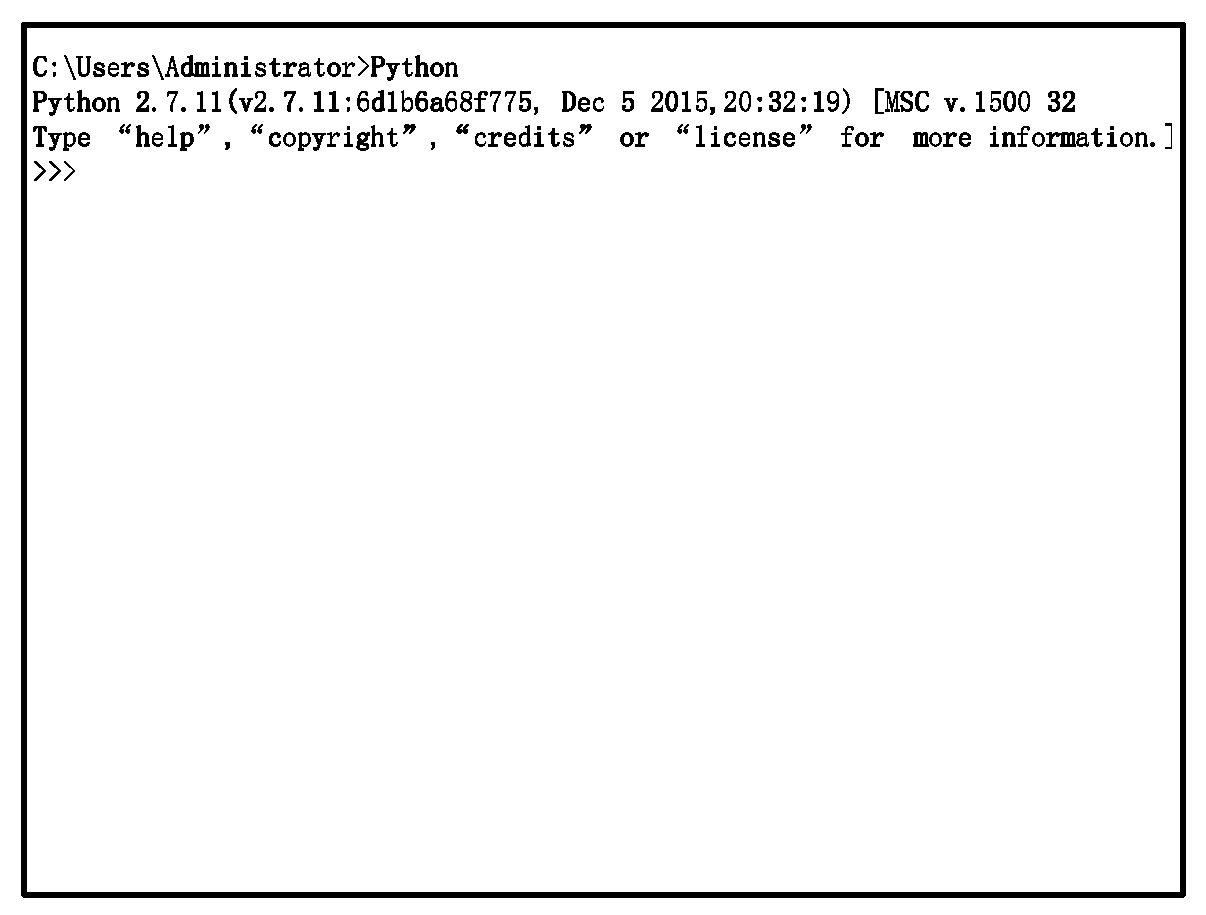
\includegraphics[width=11cm,height=8cm]{fig3_1}
\caption{Python 解释器安装成功}
\end{figure}

\section{Python\heiti 第三方库安装}
我司会为用户提供运行软件所需的所有第三方Python库的安装文件,包括wxpython、matplotlib(包括dateutil文件与pyparsing文件)、numpy、six等。下面依次讲解如何安装这4个第三方库。
\vspace{0.4cm}

\noindent$\vcenter{\hbox{\huge$\bullet$}}$\quad\fontsize{12pt}{\baselineskip}\textbf{\heiti{安装}wxpython\heiti{库}:}

进入我司为用户提供的“ASG\_install”文件夹下的wxpython文件夹,双击其中的exe安装程序,点击“Next”即可安装wxpython库。
\vspace{0.4cm}

\noindent$\vcenter{\hbox{\huge$\bullet$}}$\quad\fontsize{12pt}{\baselineskip}\textbf{\heiti{安装}matplotlib\heiti{库}:}

进入我司为用户提供的“ASG\_install”文件夹下的“matplotlib”文件夹,双击其中的exe安装程序,点击“Next”即可安装matplotlib库。安装matplotlib库后还需要安装两个文件:dateutil文件与pyparsing 文件。
\vspace{0.4cm}

\noindent$\vcenter{\hbox{\huge$\bullet$}}$\quad\fontsize{12pt}{\baselineskip}\textbf{\heiti{安装}dateutil\heiti{文件}:}

进入Windows命令行(点击任务栏“开始”按钮,输入“cmd”后按回车),然后通过DOS下的“cd”命令(切换目录),将当前目录切换到您存放我司提供的“matplotlib”文件夹所在位置。如用户将“ASG\_install”文件夹放在E盘的主目录下时,在命令窗口中依次输入“E:” → “cd ASG\_install” → “cd matplotlib”,即可将当前目录切换到存放“matplotlib”文件夹的位置。然后通过“pip install”命令来安装dateutil文件。完整过程为如图3.2,依次输入命令即可安装dateutil 文件。
\begin{figure}[ht]
\centering
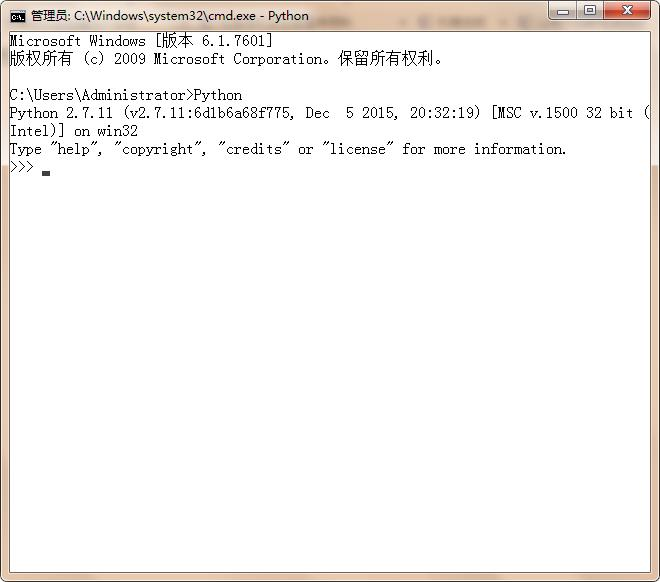
\includegraphics[width=11cm,height=8cm]{fig3_2}
\caption{安装dateutil文件}
\end{figure}

\newpage
\noindent$\vcenter{\hbox{\huge$\bullet$}}$\quad\fontsize{12pt}{\baselineskip}\textbf{\heiti{安装}pyparsing\heiti{文件}:}

同安装dateutil一样,先在DOS命令窗口将目录切换到我司提供的“matplotlib”文件夹所在位置,然后通过“pip install”命令来安装pyparsing文件。如用户将“ASG\_install”文件夹放在E盘的主目录下时,完整安装过程如图3.3。

%进入Windows命令行,然后将目录切换到您存放我司提供的“matplotlib”文件夹所在位置。如图3-3输入命令即可安装pyparsing文件。

\begin{figure}[H]
\centering
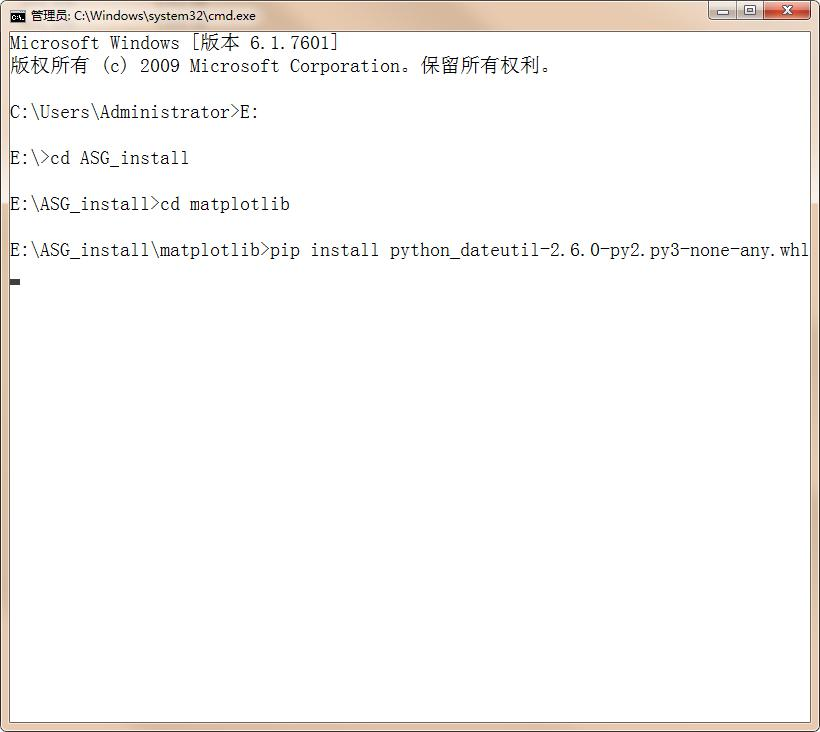
\includegraphics[width=11cm,height=8cm]{fig3_3}
\caption{安装pyparsing文件}
\end{figure}

\noindent$\vcenter{\hbox{\huge$\bullet$}}$\quad\fontsize{12pt}{\baselineskip}\textbf{\heiti{安装}numpy\heiti{库}:}

在DOS命令窗口将目录切换到存放我司提供的“numpy”文件夹所在位置,然后通过“pip install”命令来安装numpy库。如用户将“ASG\_install”文件夹放在E盘的主目录下时,完整安装过程如图3.4。
\begin{figure}[H]
\centering
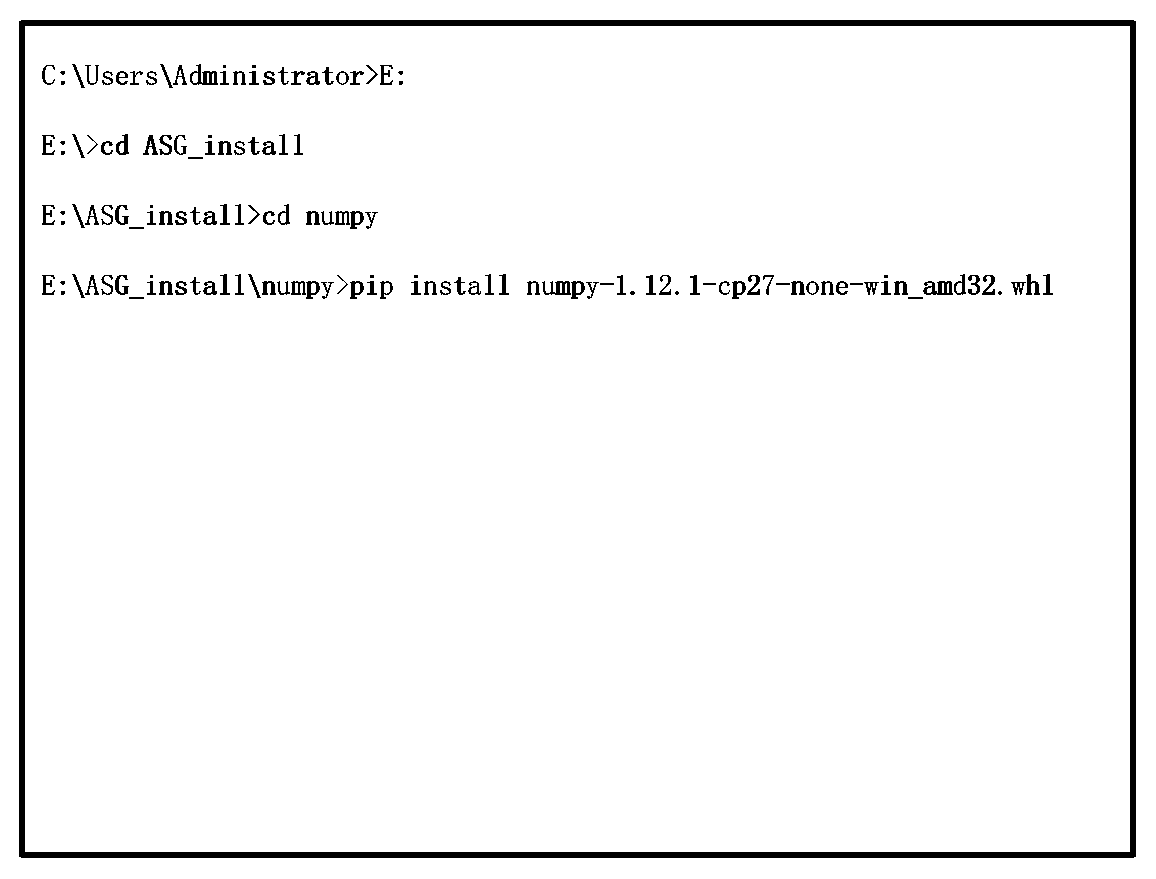
\includegraphics[width=11cm,height=8cm]{fig3_4}
\caption{安装numpy库}
\end{figure}

\noindent$\vcenter{\hbox{\huge$\bullet$}}$\quad\fontsize{12pt}{\baselineskip}\textbf{\heiti{安装}six\heiti{库}:}

在DOS命令窗口将目录切换到存放我司提供的“six”文件夹所在位置,然后通过“pip install”命令来安装six库。如用户将“ASG\_install”文件夹放在E盘的主目录下时,完整安装过程如图3.5。
%进入Windows命令行,然后将目录切换到您存放我司提供的“six”文件夹所在位置。如图3-5输入命令即可安装six库。
\begin{figure}[H]
\centering
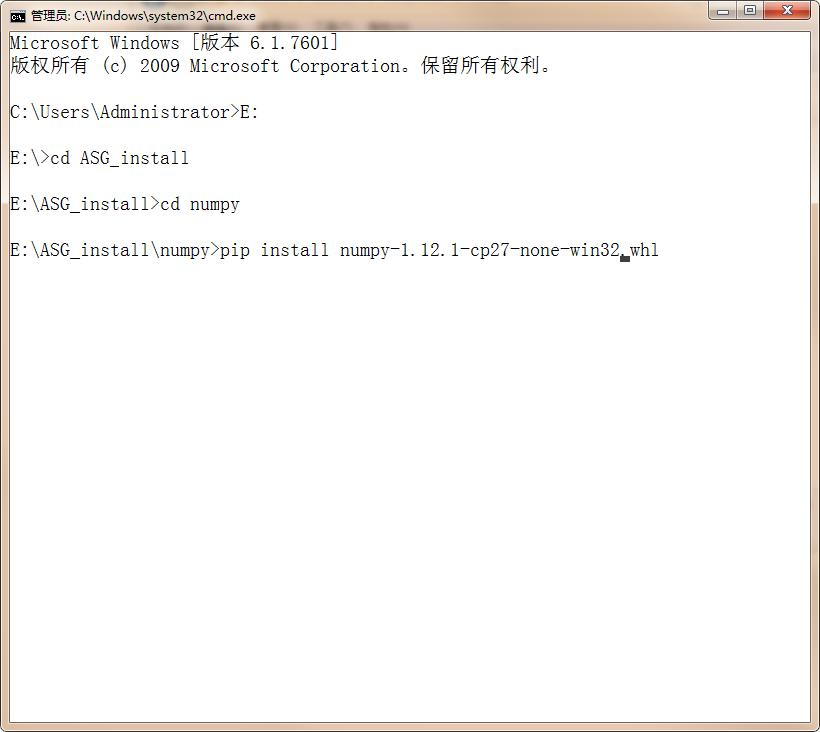
\includegraphics[width=11cm,height=8cm]{fig3_5}
\caption{安装six库}
\end{figure}

\section{USB\heiti 驱动程序安装}
在一台计算机上首次连接仪器时,系统会自动安装仪器运行所需的USB驱动程序。若自动安装失败,请打开计算机设备管理器,在“通用串行总线控制器”找到驱动未安装成功的设备,手动安装驱动程序(右键选择设备→ 更新驱动程序软件→浏览计算机以查找驱动程序软件),定位至我司为用户提供的“Drivers”文件夹即可。驱动安装成功后,在设备管理器中可以看到如图3.6所示的“Cypress FX3 USB StreamerExample Device” 被识别的状态。
\begin{figure}[htbp]
\centering
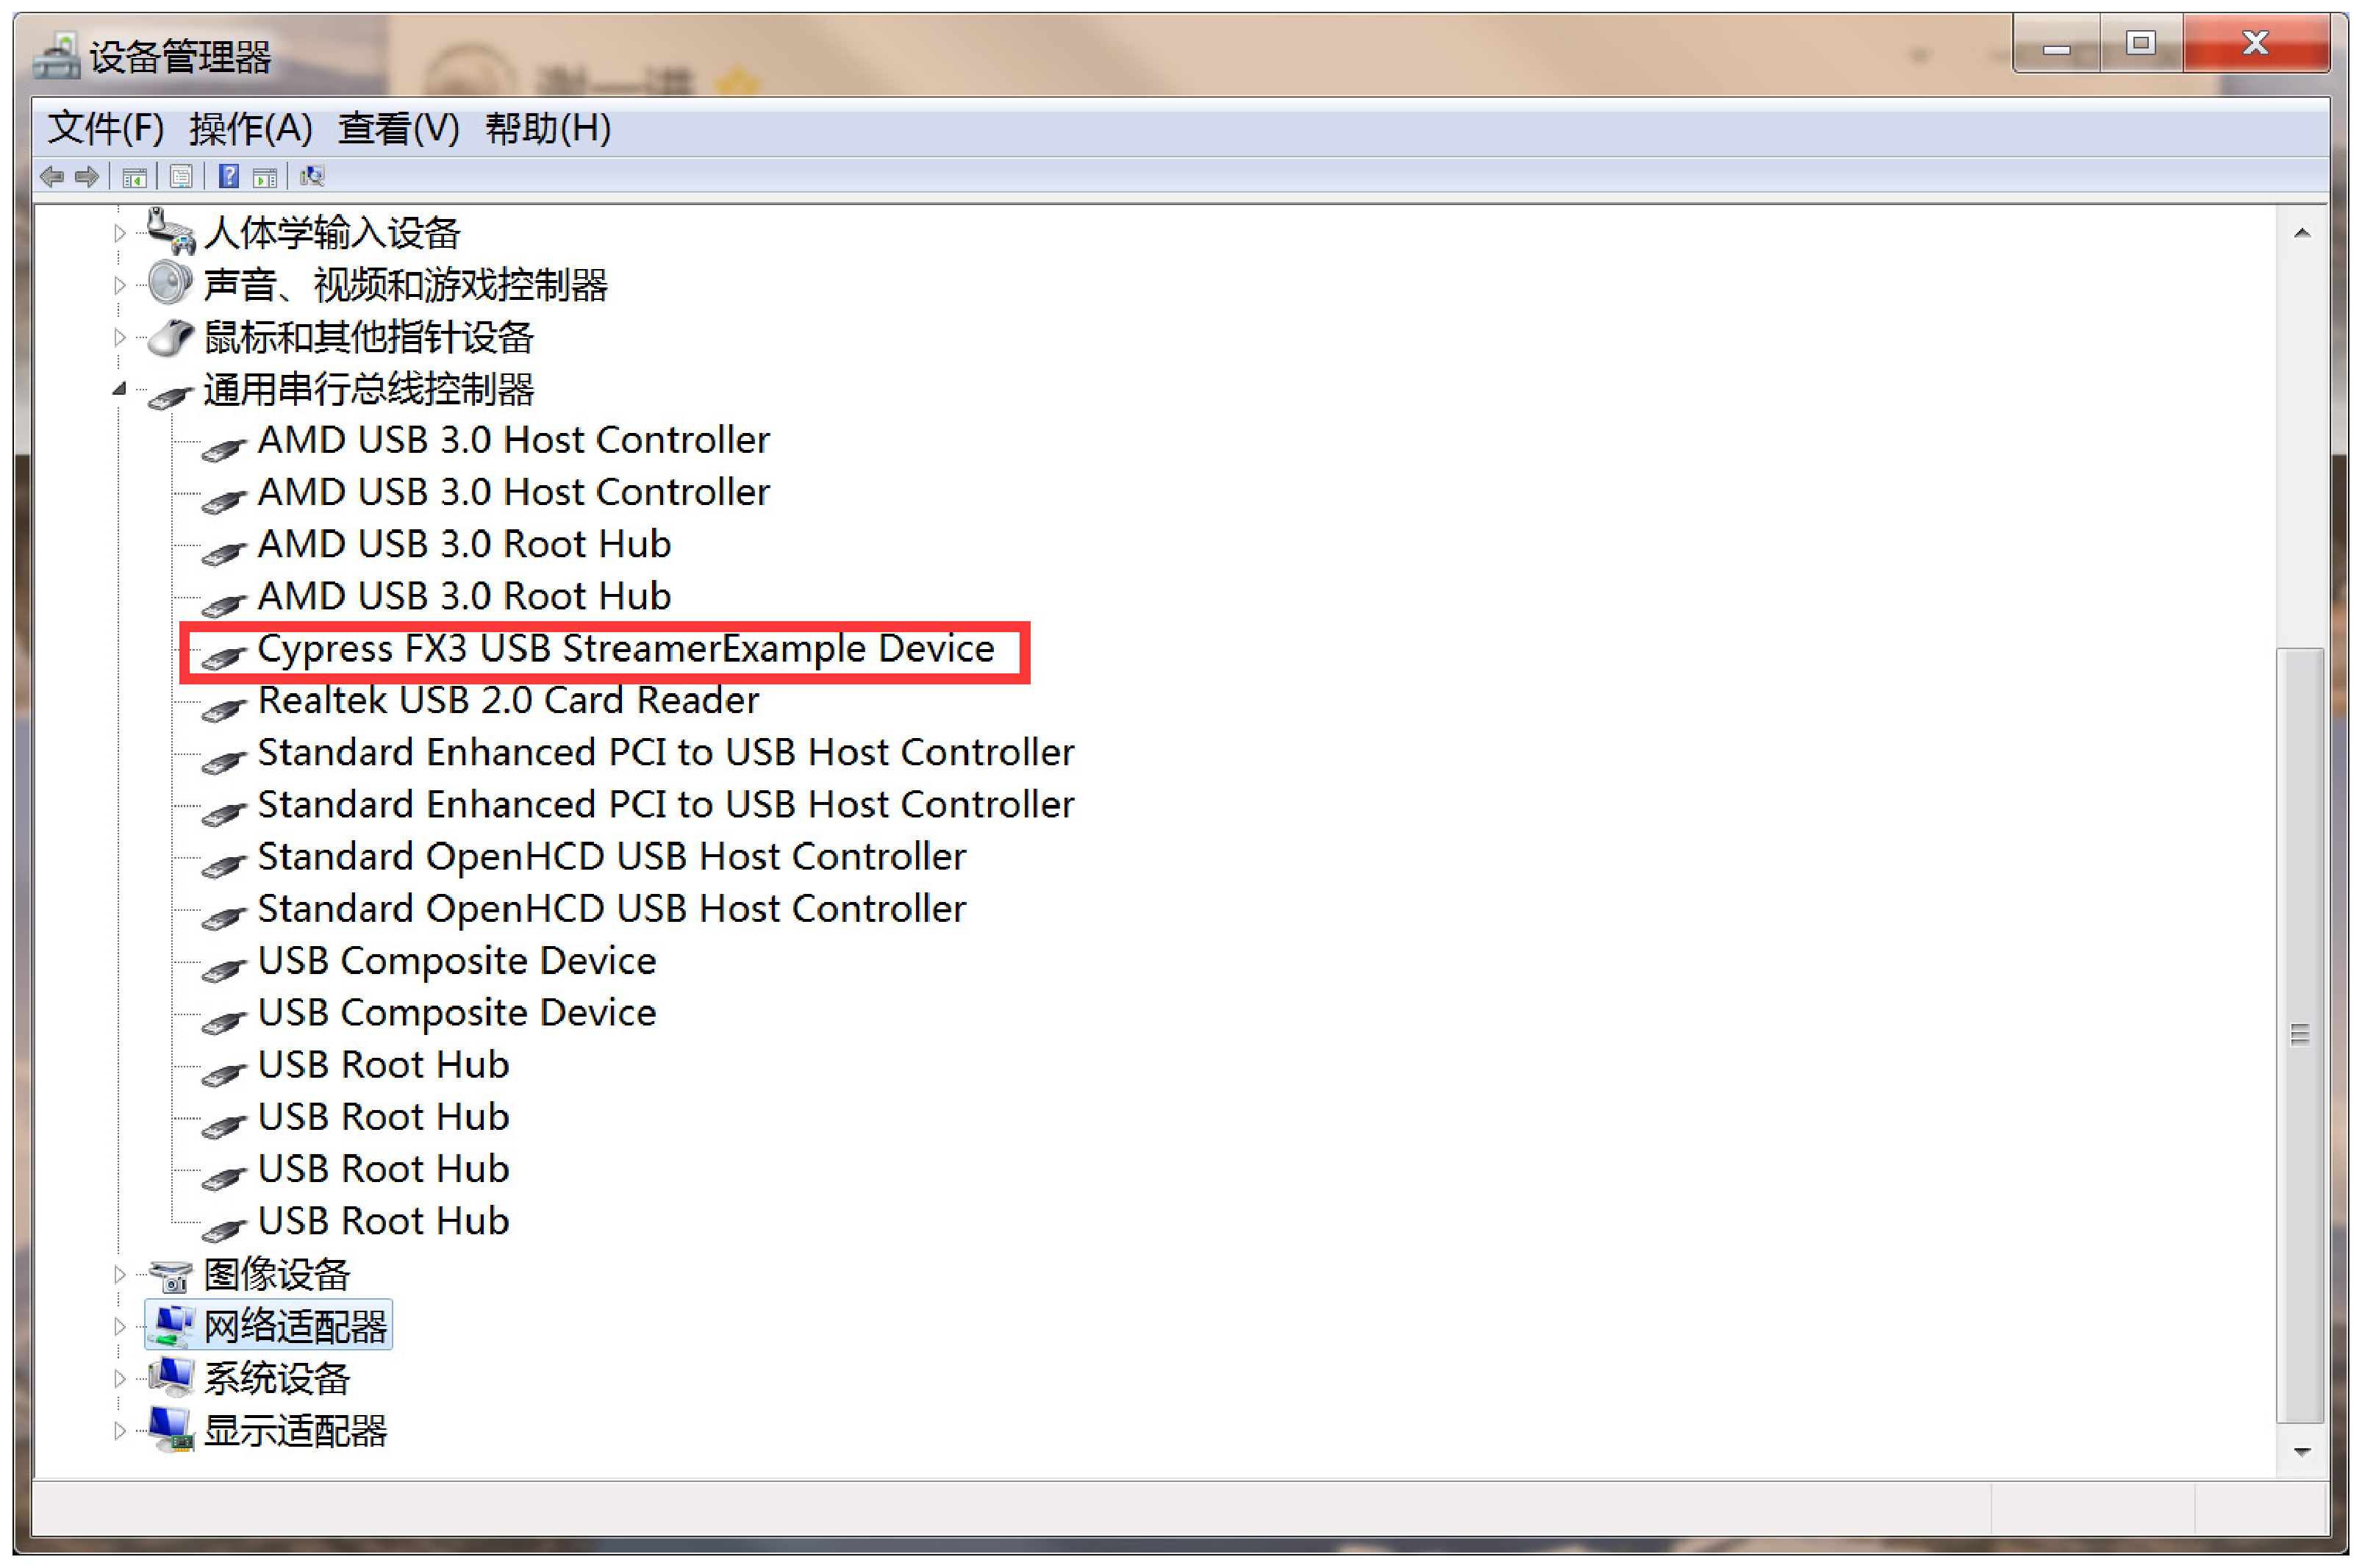
\includegraphics[width=10cm,height= 8.0cm]{fig3_6}
\caption{驱动程序安装}
\end{figure}

驱动程序安装完成后,双击“Cypress FX3 USB StreamerExample Device”打开其属性,进入“电源管理”选项。如图3.7,取消勾选“允许计算机关闭此设备以节约电源”。
\begin{figure}[htbp]
\centering
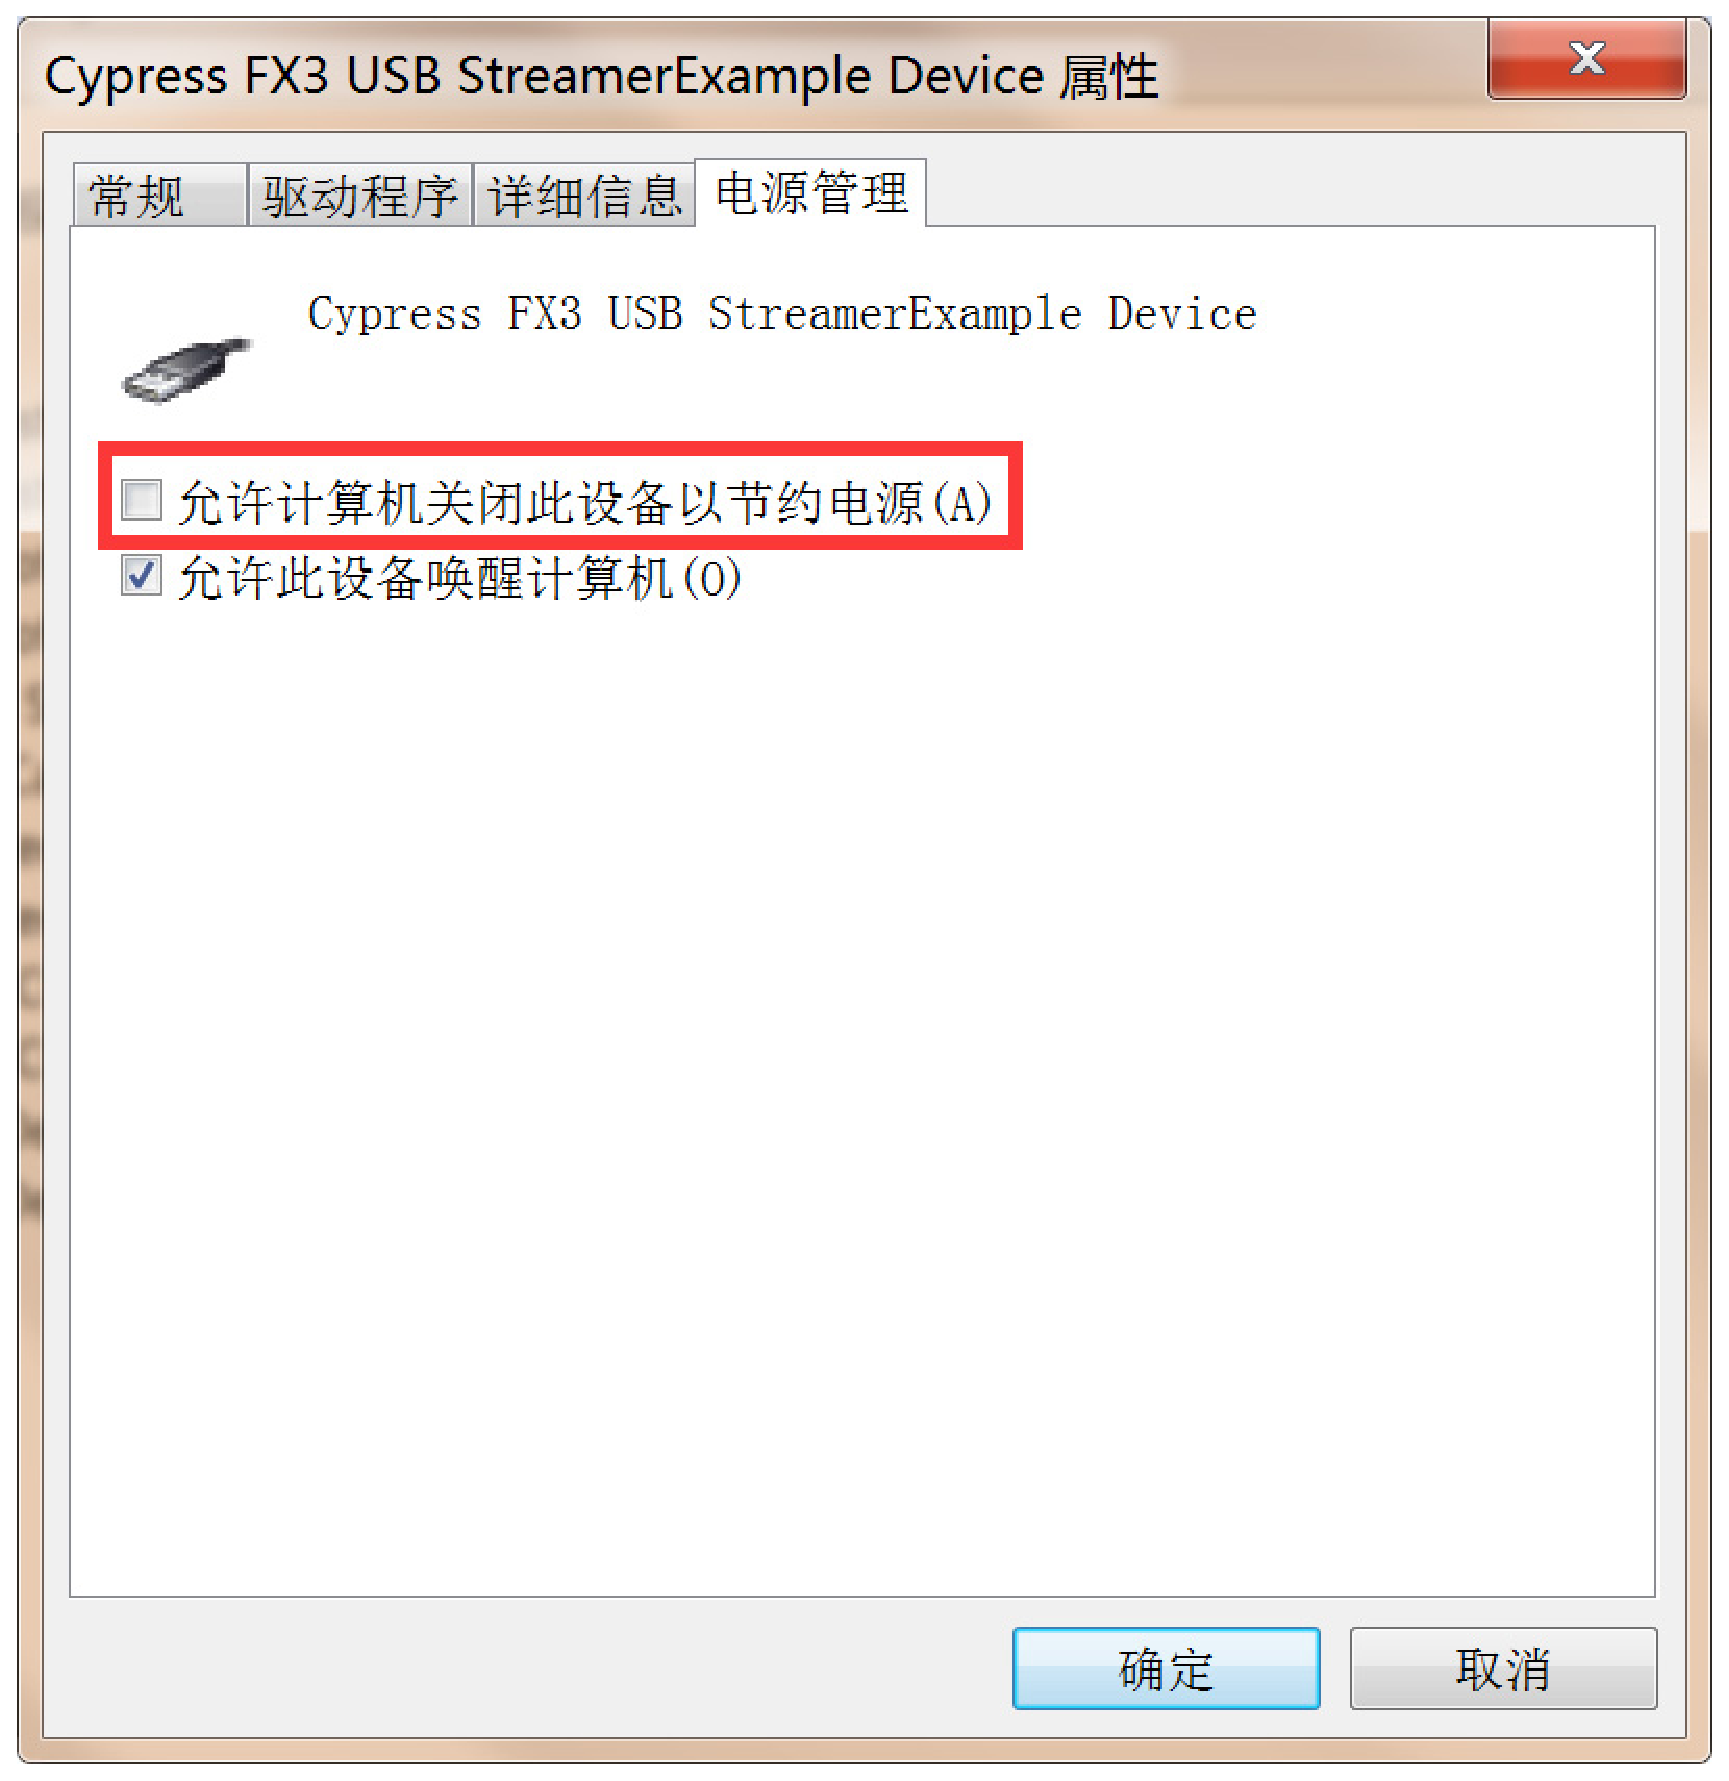
\includegraphics[width=10cm,height=8.5cm]{fig3_7}
\caption{更改电源管理选项}
\end{figure}




